\section{EDA} 
\begin{frame}{Exploratory Data Analysis - Correlation}
    \begin{columns}[T]
        \column{0.5\textwidth}
            \textbf{Analysis of the numerical variables correlation}
            \begin{itemize}
                \item Subset of relevant variables related to women labour and ECEC services
                \item Find which variables are strongly correlated, especially to the female employment rate: \\
                \begin{enumerate}[{\textcolor{deepBluePolimi}{\arabic*.}}]
                    \item per\_capita\_user\_contribution
                    \item per\_capita\_public\_expenditure
                    \item ecec\_partecipation + coverage
                \end{enumerate}
                
            \end{itemize}
    
        \column{0.5\textwidth}
        \centering
        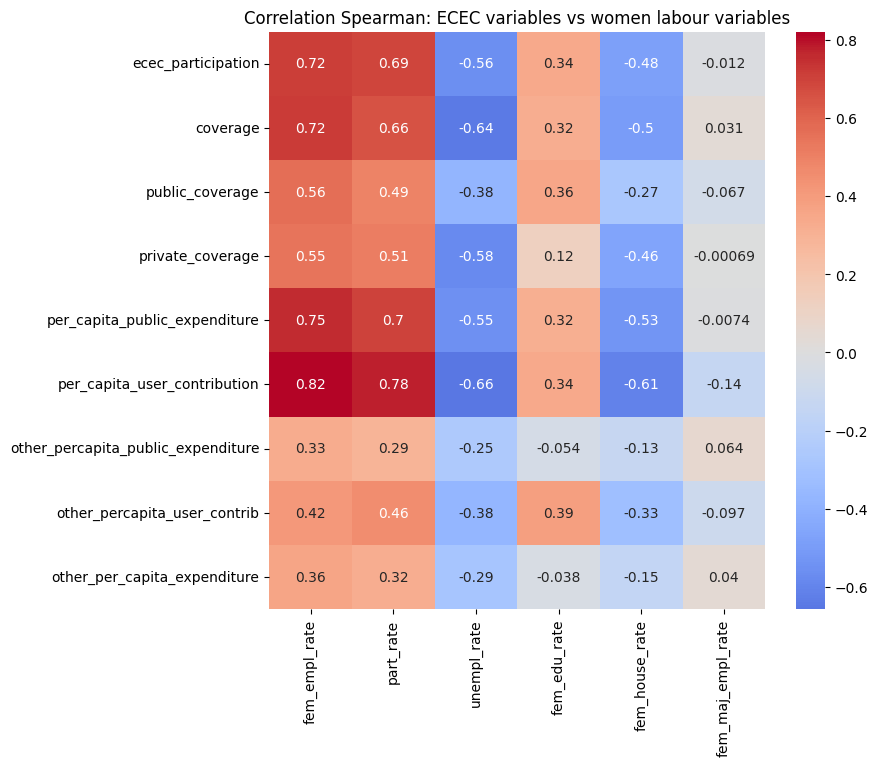
\includegraphics[width=\linewidth]{pictures/small_correlation_matrix.png}
    \end{columns}

\end{frame}

\begin{frame}{Exploratory Data Analysis - Spatial Visualization}

    \vfill
    
    \begin{center}
        Female employment rate and ECEC coverage by province
        
        \vspace{0.3 cm}
        
        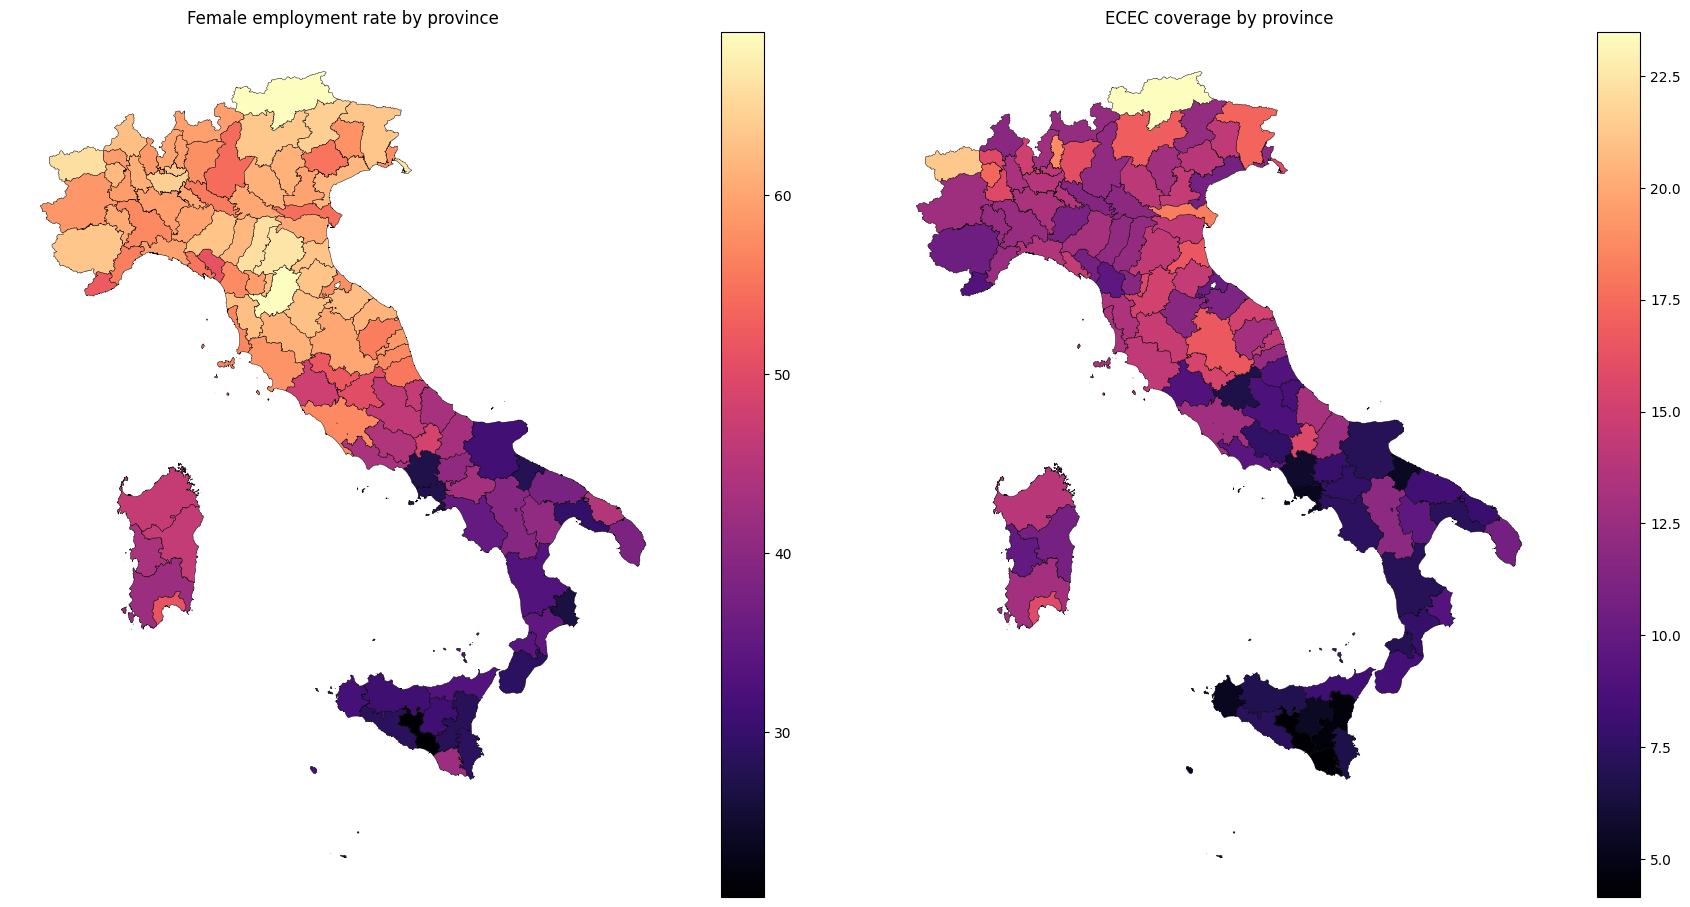
\includegraphics[width=0.72\linewidth]{pictures/fem_emp_rate_and_ECEC_map.png}
    \end{center}
    
    \vfill
    
\end{frame}


\begin{frame}{Exploratory Data Analysis - Moran's I Cluster}

    \vfill

    \begin{center}
        Female employment rate and ECEC coverage cluster
        
        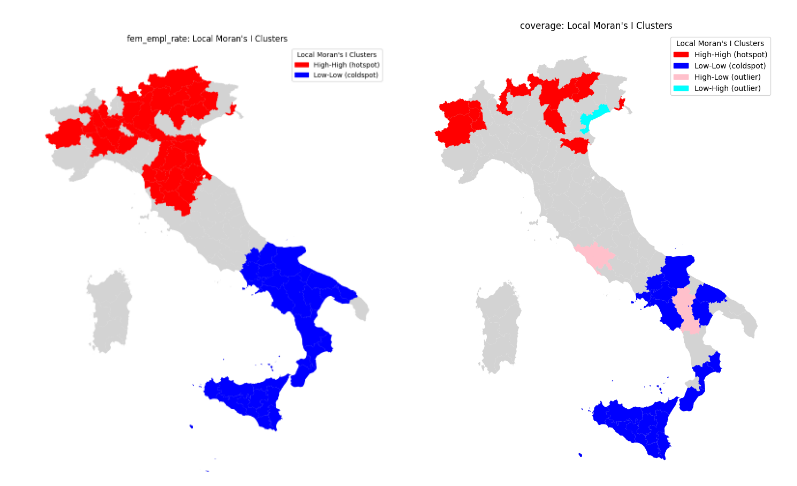
\includegraphics[width=0.7\linewidth]{pictures/morans_clusters_inverted.png}
    \end{center}

    \vfill
    
\end{frame}